\section{Sesión 17}

\begin{teorema}
	Suponga que $f_n:A\subseteq \mathbb{R}\to\mathbb{R}$ es acotada sobre $A$, $\forall n\in\mathbb{Z}^+$, y que $f_n\to f$ uniformemente sobre $A$. Entonces, $f:A\to \mathbb{R}$ es acotada sobre $A$. 
\end{teorema}

\begin{teorema}(Weiestrass)
	Suponga que $(f_n)$ es una sucesión de funciones diferenciables, 
	$$f_n:(a,b)\to\mathbb{R}\ni$$
	$f_n\to f$ puntualmente y $f'_n\to g$ uniformemente, donde $f$ y $g:(a,b)\to\mathbb{R}$. Entonces, $f$ es diferenciable sobre $(a,b)$ y $f'=g$. 
\end{teorema}

\begin{definicion}
	Sea $(f_n)$ una sucesión de funciones en $A\subseteq \mathbb{R}$. 
	\begin{enumerate}
		\item Se dice que $(f_n)$ es creciente, si $f_n(x)\leq f_{n+1}(x), \forall n\in \mathbb{Z}^+$ y $\forall x\in A$. 
		\item Se dice que $(f_n)$ es decreciente si $f_n(x)\geq f_{n+1}(x)$, $\forall n\in \mathbb{Z}^+$ y $\forall x\in A$. 
		\item Si $(f_n)$ es creciente o decreciente, entonces $(f_n)$ es monótona. 
	\end{enumerate}
\end{definicion}

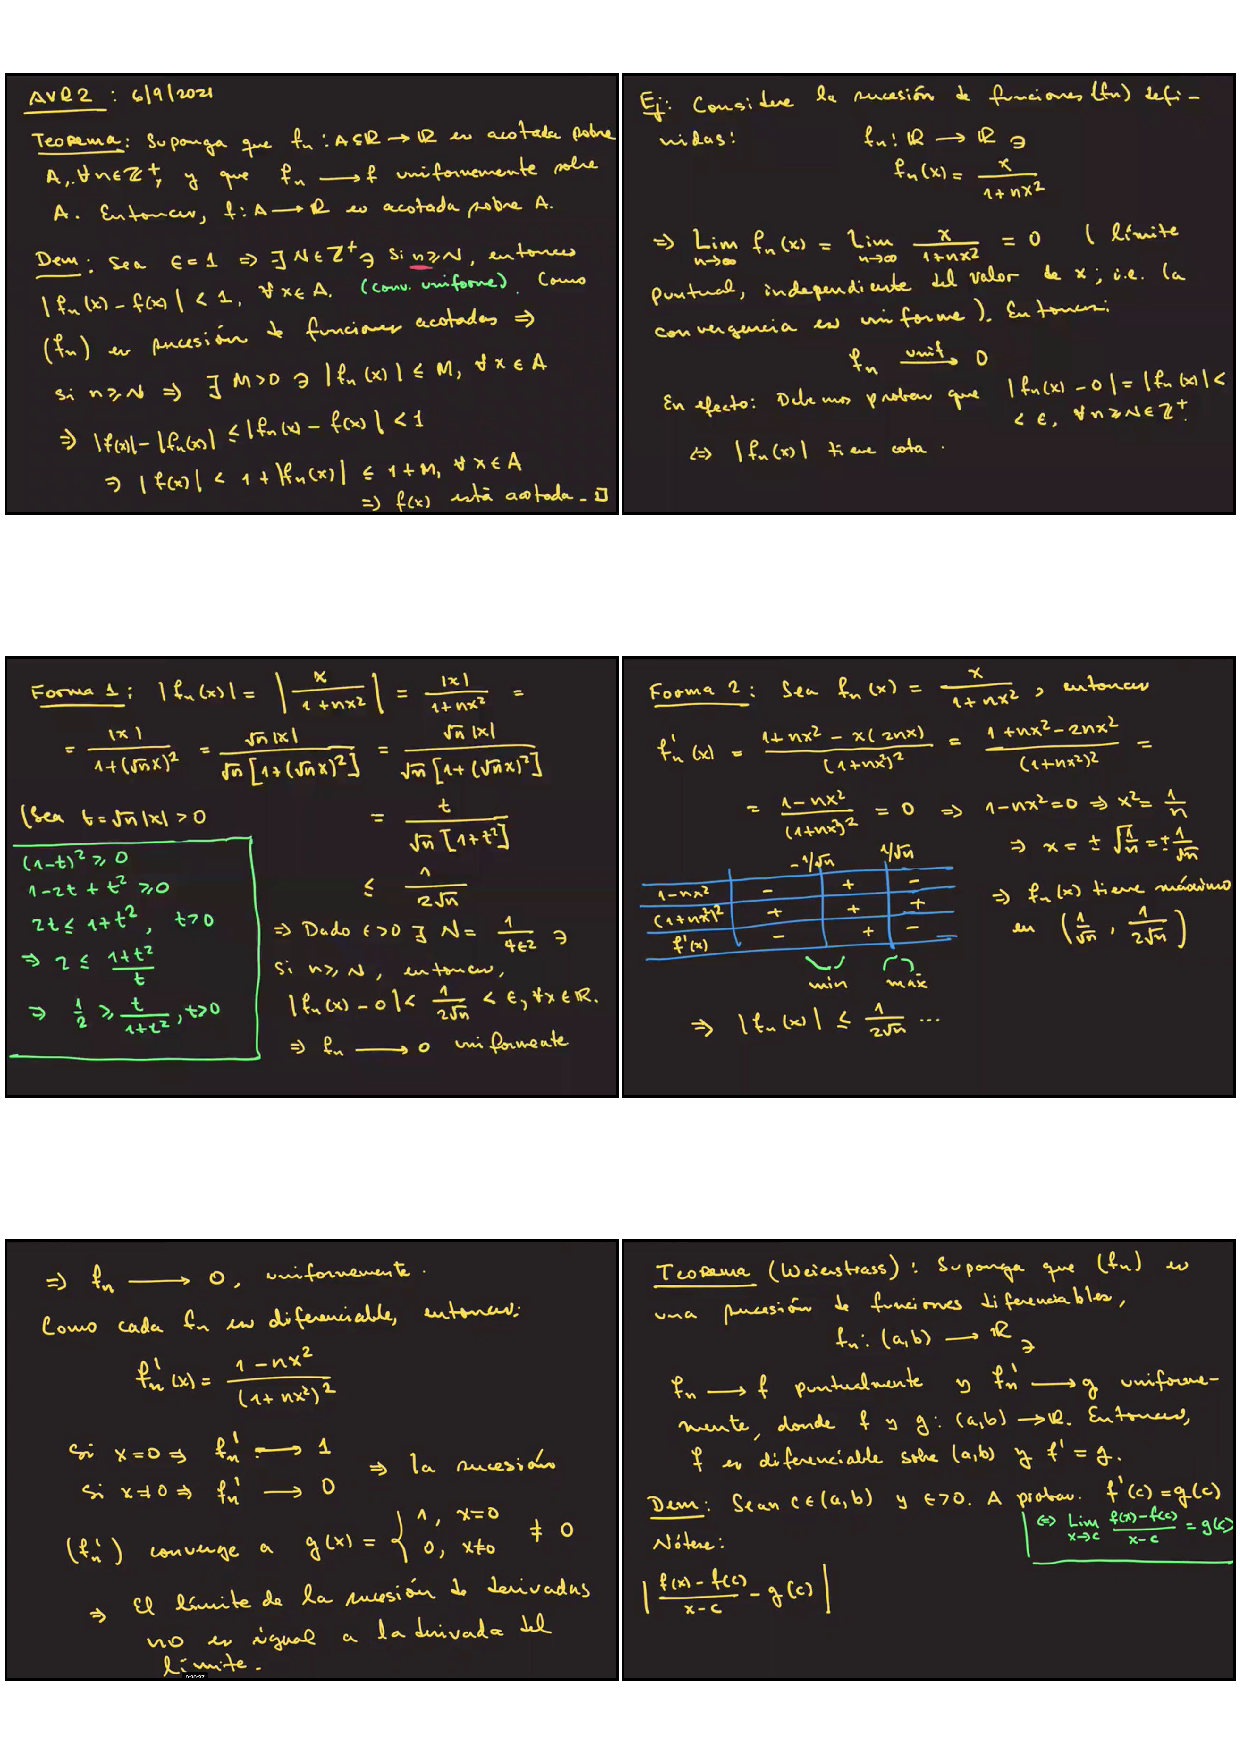
\includepdf[pages=-]{apendices/s17.pdf}